\subsection{其他的结构}
前一节假设了最简单的聚合物结构-线性均聚物。对于各种各样的体系结构包括那些具有实际和学术意义的都可以得到类似的结果。在本节中,我们导出了在空间变化势作用下分支均聚物(branched homopolymers)、嵌段共聚物和接枝共聚物(block and graft copolymers)的显式表达式。假定结构关于具有化学无序的聚合物,如随机支化均聚物(randomly branched homoploymers)、统计共聚物(statistical copolymers)和随机接枝共聚物(randomly grafted copolymers)的讨论,将推迟到4.7节讨论。
\subsubsection{分支均聚物}
作为分支均聚物的第一个例子,我们考虑一个$3$星聚合物,如图$(3.4)$所示。每个臂采用连续高斯链模型描述,相应的,每条链的聚合度分别是$N_1$,$N_2$,$N_3$。假设每个臂上的片段经历一个化学势场$w \mathbf{r}$。在这种情况下只需要一种化学势,因为臂在化学上是相同的。
\begin{figure}[H]
\centering
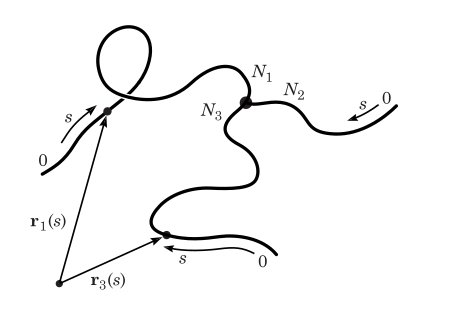
\includegraphics[scale=0.7]{./figures/34.png}
\caption{}
\end{figure}
图$(3.4)$连续高斯链模型中的$3$星聚合物。聚合度分别为$N_1$,$N_2$,$N_3$的三个支臂连接在一个中心支点上。第$j$个臂的构型用空间曲线$\mathbf{r}_j(s)$描述,$s\in [0,N_j]$。

如图$(3.4)$所示,第$j$个臂$(j=1,2,3)$的构型由空间曲线$\mathbf{r}_j(s)$描述,其中路径参数$0\leq s\leq N_j$,这是从每个臂的自由端测量。支点臂的约束条件为$\mathbf{r}_1(N_1)=\mathbf{r}_2(N_2)=\mathbf{r}_3(N_3)$。

第$3.1.2$节关于线性均聚物的公式可以很容易地推广到目前的情况。微观段密度(microscopic segment density)可以写成
\begin{gather}
\rho(\mathbf{r})=\sum_{j=1}^3 \int_0^{N_j}\, \mathrm{d}s\rho(\mathbf{r}-\mathbf{r}_j(s))
\end{gather}
与施加的化学势$w \mathbf{r}$的势能的函数与聚合物整体构型$\mathbf{r}(s)\equiv \left\{ \mathbf{r}_1(s),\mathbf{r}_2(s),\mathbf{r}_3(s) \right\}:$
\begin{gather}
\beta U_1[\mathbf{r},w]=\int \mathrm{d}\mathbf{r}^{'}w(\mathbf{r}^{'})\rho(\mathbf{r}^{'})
\end{gather}
归一化的配分函数$Q[w]$也可以表示为路径积分的比率
\begin{gather}
Q[w]\equiv \frac{Z[w]}{Z_0}=frac{\int^{*}\mathcal{D}\mathbf{r}\exp (-\beta U_0[\mathbf{r}]-\beta U_1[\mathbf{r},w])}{\int^{*}\mathcal{D}\mathbf{r}\exp (-\beta U_0[\mathbf{r}])}
\end{gather}
其中理想链的势能
\begin{gather}
\beta U_0[\mathbf{r}]=\frac{3}{2b^2}\sum_{j=1}^3\int_{0}^{N_j} \mathrm{d}s\left| \frac{d\mathbf{r}_j(s)}{ds} \right|^2
\end{gather}
和$\int^{*}\mathcal{D}\mathbf{r}$是受支点约束的三个臂上的路径积分
\begin{gather}
\int^{*}\mathcal{D}\mathbf{r}\equiv \int \mathcal{D}\mathbf{r}\delta (\mathbf{r}_1(N_1)-\mathbf{r}_2(N_2))\delta (\mathbf{r}_2(N_2)-\mathbf{r}_3(N_3))
\end{gather}
方程$(3.82)$中的路径积分可以通过离散这三条路径来计算,这三条路径对应于星臂的构型,从而得到了一个类似于线性均聚物方程$(3.21)$的表达式。方程$(3.84)$的约束是通过建立三个臂从自由端开始,在公共分支点的位置终止的路径积分,因此,由乘积$q(\mathbf{r},N_2;[w])q(\mathbf{r},N_3;[w])$给出了在支点为$\mathbf{r}$的星形聚合物的统计重量,其中(propagators)满足方程$(3.25)-(3.26)$。配分函数是
\begin{gather}
Q[w]=\frac{1}{V}\int \mathrm{d}\mathbf{r}~q(\mathbf{r},N_1;[w])q(\mathbf{r},N_2;[w])q(\mathbf{r},N_3;[w])
\end{gather}
%应该注意,应用这个公式并不需要扩散方程$(3.25)$的三个独立解,而是一个,因为对$0\leq s\leq N_{\max}$(其中$N_\max$是$N_j$中最大的)的$q(\mathbf{r},s;[w])$足以评估全部的三个传播子。

$3$星形均聚物的段密度算子可与线性聚合物的方程$(3.55)$类比得出。在连续高斯链模型中,我们有
%\begin{gather}

%\end{gather}












%\begin{gather}

%\end{gather}

%\begin{gather}

%\end{gather}